\documentclass{llncs}

\usepackage{graphicx}
\usepackage{url}
\usepackage{courier}
\usepackage{listings}


%!TEX root = ./paper1.tex

\lstset{
  float=tb,
	captionpos=b,
	breaklines=true,
	xleftmargin=20pt,
	basicstyle=\ttfamily\scriptsize,
	numberstyle=\tiny,
	flexiblecolumns=true,
	numbers=left,
	nolol=false,
	tabsize=2
}

\lstdefinelanguage{OCL}{
morekeywords={import,if,then,else,endif,self,and,true,false,def,includes,OclElement,package,let,in},
sensitive=true,
morecomment=[l]{--},
morestring=[b]",
morestring=[b]',
showstringspaces=false
}

\lstdefinelanguage{QVTo}{
morekeywords={import,modeltype,uses,transformation,inout,in,out,configuration,property,main,var,if,then,else,endif,map,new,self,library,helper, mapping, and,return, when, where, object, true, false, result},
sensitive=true,
morecomment=[l]{--},
morecomment=[l]{//},
morestring=[b]",
morestring=[b]',
showstringspaces=false
}

\lstdefinelanguage{Acceleo}{
morekeywords={template, file, if, else, for},
sensitive=true,
morecomment=[l]{--},
morecomment=[l]{//},
morestring=[b]",
morestring=[b]',
showstringspaces=false
}

\lstdefinelanguage{MWE}{
morekeywords={module, import, var, true, false, },
sensitive=true,
morecomment=[l]{//},
morestring=[b]",
showstringspaces=false
}

\lstdefinelanguage{Java}{
morekeywords={class, private, public, true, false, new, if, for, int, return, void, extends, implements, this, null, super, import, package},
sensitive=true,
morecomment=[l]{//},
morestring=[b]",
showstringspaces=false
}

\lstdefinelanguage{JastAdd}{
morekeywords={abstract, ast, syn, inh, eq, boolean, int, false, true, if, for, return},
morestring=[b]',
sensitive=true
}

\lstdefinelanguage{NaBL}{
morekeywords={rules, defines, unique, non, refers, to},
sensitive=true
}

\lstdefinelanguage{Gra2Mol}{
morekeywords={rule, from, to, queries, mappings, skip, end_rule},
morestring=[b]',
sensitive=true
}

\lstdefinelanguage{Xtext}{
morekeywords={terminal, returns, grammar, import, fragment, current},
morestring=[b]',
morecomment=[l]{//},
sensitive=true
}

\lstdefinelanguage{Xtend}{
morekeywords={FOR, ENDFOR, IF, ELSE, ENDIF, def, protected, void, new, var, typeof, return},
morestring=[b]',
morestring=[b]",
morecomment=[s]{/*}{*/},
sensitive=true
}

\lstdefinelanguage{CS2AS}{
morekeywords={source, target, nameresolution, named, element, exports, for, from, all, children, resolution, helpers, mappings, map, disambiguation, lookup, lookupFrom, resolve, trace, when, occluding, nested,scope, def, protected, import,if,then,else,endif,self,and,true,false,def,includes,OclElement,package,let,in, void, new, var, typeof, return},
morestring=[b]',
morestring=[b]",
morecomment=[s]{/*}{*/},
sensitive=true
}



\begin{document}


\title{Technical Obsolescence Management Strategies for Safety-Related Software for Airborne Systems -- Assurance Report}

\author{Richard F. Paige\inst{1}, Simos Gerasimou\inst{1} and Dimitris Kolovos\inst{1}}

\institute{
Department of Computer Science, University of York, UK.\\
\email{[richard.paige,simos.gerasimou,dimitris.kolovos]\_at\_york.ac.uk}
}
\maketitle

\begin{abstract}
This report briefly summarises the technical challenges associated with certification (and re-certification)
of software after a particular obsolescence management strategy -- described in a companion report -- has
been carried out. In particular, it firstly considers the types of evidence that can
be produced by the management strategy. Secondly, it considers the DO-178B objectives and analyses where specific objectives
may need to be reconsidered in order to achieve re-certification. In this manner it aims to demonstrate where
re-certification effort may need to be prioritised.Finally, it briefly comments on two issues: qualification of tools that support
the management strategy, and automatic generation of certification cases, which may help to reduce the amount of effort 
required in supporting re-certification.
\end{abstract}

\section{Introduction}
Complex software systems deployed in safety-critical and business-critical 
application domains (e.g., avionics, defence, healthcare) are meant to provide 
service for decades. Although many of these systems withstand technological 
evolution and infrequently undergo substantial changes, they will likely face 
software obsolescence problems during their lifetime. 
Resolving these obsolescence problems is an expensive, time-consuming and 
labour intensive process. The costs

In this project, we explore reactive strategies for managing software 
obsolescence in safety-related software for airborne 
systems~\cite{ProjectResponse}. More specifically, we 
investigate the extent to which \textit{software modernisation} -- i.e., 
approaches that involve changes to the system 
structure, adaptation to more advanced technologies, and functionality 
enhancement -- can mitigate the problem of software obsolescence and extend the 
life, performance and reliability of existing systems. We adopt an 
experimental-based approach and use a set of demonstrators to explore different 
facets of software modernisation, 
including reverse engineering, program understanding, demonstration of 
functional equivalence of 
migrated code, change in hardware platform, maintenance of performance, and 
preservation of Design Assurance Levels (DAL).

In this report we focus on certification and assurance issues, specifically: if the obsolescence management strategy
presented in the companion report is applied to a system at DAL-C, what are the certification issues associated with
the migrated software? In particular, what effort will be required to re-certify the software system, and what evidence
can the strategy provide in order to support re-certification?

The emphasis in this 11-month project sponsored by DSTL has been on building and evaluating a technical solution to
software obsolescence on several case studies; assurance and certification has been a secondary concern. As such, this
report is primarily speculative. It is structured as follows. Firstly, we describe the evidence that is produced by the 
obsolescence strategy and technical solution that is relevant to certification and recertification. We also briefly describe
the toolchain that has been developed to support the obsolescence strategy, so that the report is moderately self-contained
and hence easier to follow. Next, we analyse the DO-178B objectives and summarise which specific objectives \textit{must} and
\textit{could} be reconsidered as a result of applying the strategy. Finally, we comment on two issues: that of tool qualification
(and the challenges that will arise in qualifying the toolchain developed within this project), and of automatically generating 
assurance/safety cases from the engineering artefacts that are provided as input to the obsolescence strategy.

\section{Background and Evidence}
In this section, we briefly describe the technical solution that has been developed to help support an obsolescence management
strategy. The solution and the obsolescence management strategy is described in more detail in the accompanying report \cite{Gerasimou2017}. 
We also briefly describe the evidence that is produced by following the strategy and using the technical approach.

\subsection{Technical approach summary}
Technological obsolescence problems
include end-of-support of a crucial software component (which is part of a 
software system) that enforces adaptation to more advanced technologies, and 
the 
need to transform parts of a software system developed in a ``legacy'' 
programming language to a modern programming language (e.g., from Ada to 
C/C++). 
A common, but challenging, functional obsolescence problem  of interest 
involves the migration of an entire software system from a legacy hardware 
platform to a modern, more powerful platform.

Resolving these software obsolescence problems is typically a manual and laborious process. We have explored techniques to enable the partial 
automation of reactive mitigation strategies, targeting mainly C/C++ software 
systems. In particular, we proposed a combination of code analysis, code-based 
transformation and verification/validation techniques for the 
\textit{modernisation} of software systems.
Figure~\ref{fig:approach} depicts an overview of the proposed approach to 
software modernisation. 

\begin{figure}[htbp]
	\vspace*{-2em}
	\centering
	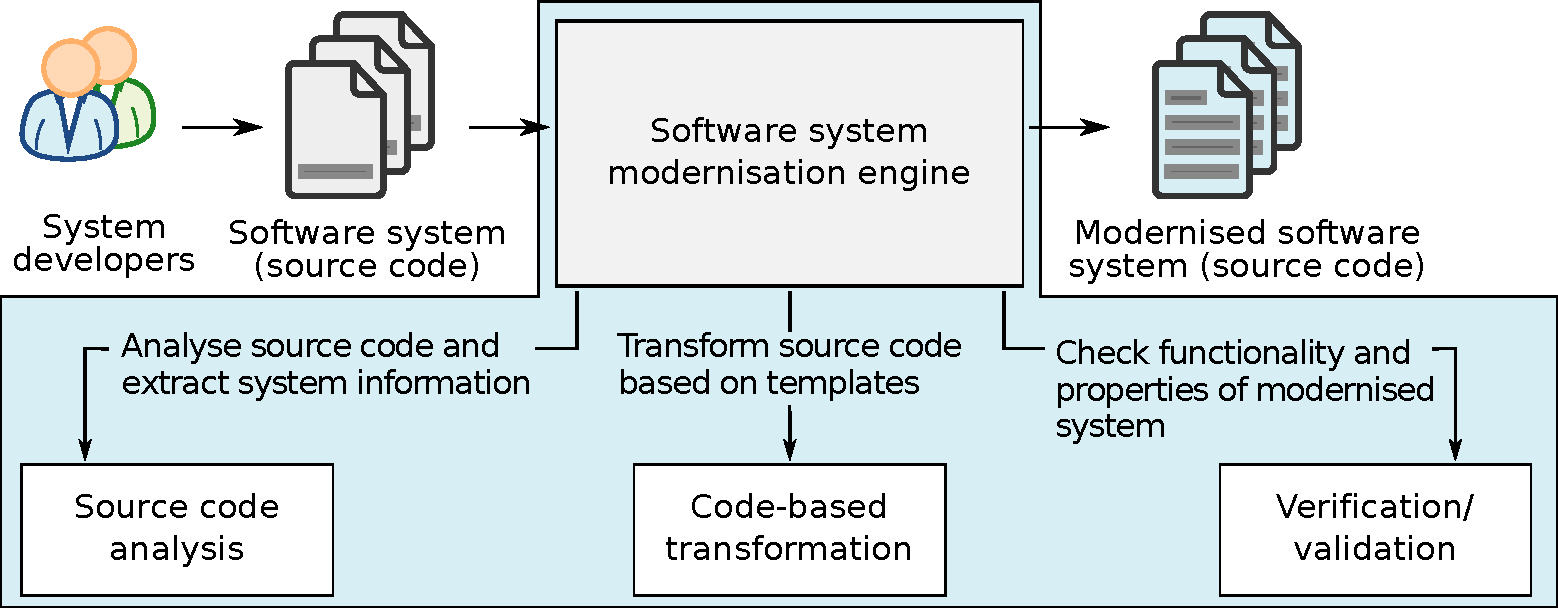
\includegraphics[width=.9\linewidth]{figures/architecture.pdf}
	
	\caption{High-level software modernisation approach.}
	\label{fig:approach}
	
	\vspace*{-2em}
\end{figure}

Through analysing the source code of the software system under consideration, 
we would gain insight into the architecture of the system, including 
interconnections between software modules and dependencies with 
external libraries and components. Furthermore, this code analysis will provide 
useful information on how to best address the obsolescence issues and 
re-architect the software, if needed.

The approach illustrated in Figure~\ref{fig:approach} is based on the use of transformation technology.
Two types of transformations have been used to support rehosting: extraction 
transformations (to “pull” abstract specifications from legacy code) and text 
generators, based on templates. The transformations have been implemented using Epsilon, the rich C/C++ parsing and analysis 
infrastructure provided by the Eclipse CDT project, and ANTLR/Xtext to support 
additional languages 
such as Ada. The former for implementing the templates, the latter to extract 
abstract specifications from legacy code, in a form suitable for re-engineering 
and amenable to application of the templates. 
The transformation chain will automatically generate traceability 
information in a standard format (e.g., XML-based). Such information will be potentially useful as
evidence that the rehosted/migrated application would be supportive of Software Level C.
In particular, it could used to demonstrate a partial validity argument, 
i.e., that all statements and expressions in the legacy program are transformed 
to statements and expressions in the retargeted program. 

\subsection{Evidence}
The obsolescence management strategy makes use of a number of techniques to support software migration and rehosting.
These techniques are underpinned by a number of engineering artefacts that can either be used directly as evidence in assurance, or
can be used to \textit{generate} evidence that can be used to support assurance, of the migrated or rehosted software system. 
We are assuming that we are migrating a system that has already undergone some level of certification or assurance,
e.g., against DO-178B or similar standards, to DAL-C or similar. As such, some assurance evidence already exists.

The sources of evidence available to or generated by the obsolescence management strategy and technical approach are as follows.

\begin{itemize}
\item \textit{Tests}: test cases and test evidence will have been produced for the original certification and assurance. Migration and rehosting
is designed to ensure that the migrated software system is behaviourally equivalent (modulo behavioural differences in the hardware platform).
As such, the migrated and rehosted system should satisfy the original test cases.

\item \textit{Traceability}: the technical approach we have developed generates (as a side-effect) traceability information between the original
source program and the target program. In this way, information capturing how source statements have been replaced with target statements has
been captured. This information can be externalised and used to support impact analysis, which in turn will provide information to safety engineers as
to (a) which parts of the software system have changed; (b) which parts have not changed; and (c) where they may need to concentrate their efforts
in re-certifying. Note that traceability information is \textit{static} and \textit{syntactic:} it captures the fact that program statements have been 
transformed into new program statements, but says nothing about the meaning of the transformation.

\item \textit{Transformations:} the rehosting/migration technical approach makes use of transformations and text generation algorithms, which have
been tested and can be further audited and reviewed, in much the same way as a compiler can be tested and reviewed and ultimately qualified (though in Section~\ref{sec:future}
we briefly discuss some of the challenges of qualifying migration tool chains like the one we have developed).
\end{itemize}

In the next section we briefly discuss the impact of migration on relevant safety standards -- particularly DO-178B -- and analyse the effect of migrating
a software system using the technical approach on any previously existing safety argument and safety process.

\section{Certification and DO-178B Objectives}

\section{The Future: Tool Qualification and Assurance Case Generation}

\section{Conclusions}

\bibliographystyle{abbrv}
\bibliography{bibliography}
\renewcommand{\baselinestretch}{1.0}


\end{document}